\chapter{Implementação}
Para o desenvolvimento do projeto, houveram uma série de reuniões onde o objetivo era delimitar e estabelecer alguns requisitos para a implementação do projeto, que de suma relevância para o andamento e funcionamento dos setores a serem implantados.

Para o desenvolvimento foi estabelecido uma média de 30 dias de implementação direta no desenvolvimento do projeto, considerando que a data prevista para a entrega final do projeto será em 2020/2.

\section{Tecnologias}
Para o desenvolvimento do sistemas, foram divididas em três aplicações: uma visando a parte WEB, outra visando dispositivos móveis com os sistemas Android e IOS e para efetuar a comunicação entre os sistemas e o banco dados, foi elaborado uma aplicação de servidor cujo valida as requisições e efetua a comunicação entre as aplicações visíveis e o banco de dados.
\subsection{Aplicação WEB}
Para o desenvolvimento foi utilizada as tecnologias pré requisitadas pela empresa Duas Rodas, sendo elas HTML5, SCSS e como complemento, utilizamos o TypeScript com o framework Angular 7.
\subsection{Aplicação Mobile}
Conduzido paralelamente com o desenvolvimento das demais aplicações, o sistema Mobile tem como objetivo a mobilidade, facilidade de acesso e interação podendo ser utilizado em qualquer lugar dentro da empresa.

\subsection{Aplicação do Servidor}
A aplicação do servidor é o canal centralizador das demais plataformas. Ela tem acesso único e exclusivo ao banco de dados. É responsável por todas as validações e executa regras de negócio. Nela foi utilizada a biblioteca \textit{Express} para o desenvolvimento da \textit{API} e para comunicação com o banco de dados foi utilizado a \textit{ORM Sequelize}.

\section{Códigos}

\newpage
\subsection{Mapeamento do Banco de Dados com TypeOrm}

\begin{figure}[htb]
	\caption{\label{code_server_type-orm}Mapeamento do Banco de Dados com TypeOrm}
	\begin{center}
		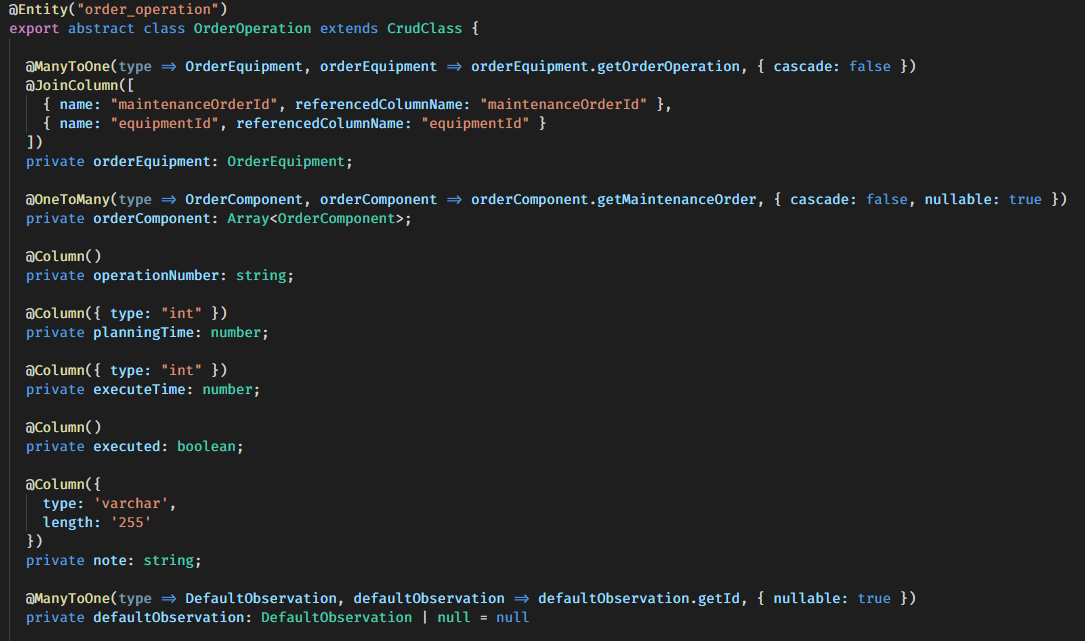
\includegraphics[scale=0.60]{./Figuras/code/server/type-orm.png}
	\end{center}
	\legend{Fonte: Próprio Autor, 2019}
\end{figure}

A figura \ref{code_server_type-orm} demonstra a utilização da TypeOrm, onde na definição de classe é possível mapear as colunas e relações das tabelas no banco de dados.

\newpage
\subsection{Validação de Objetos com o Class Validator}

\begin{figure}[htb]
	\caption{\label{code_server_class-validator}Validação de Objetos com o Class Validator}
	\begin{center}
		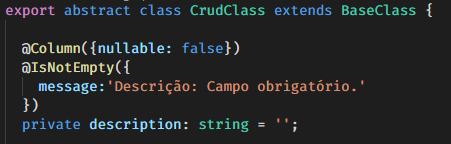
\includegraphics[scale=1.30]{./Figuras/code/server/class-validator.png}
	\end{center}
	\legend{Fonte: Próprio Autor, 2019}
\end{figure}

Na figura \ref{code_server_class-validator} é possível ver o mapeamento de uma classe com o \textit{decorator} ''IsNotEmpty'' na propriedade ''description''. Esse \textit{decorator} irá validar se a propriedade está vazia ou não, caso esteja vazia, irá retornar o erro ``Descrição: Campo obrigatório.'' conforme definição no próprio \textit{decorator}.

\subsection{Controller: Validação do Objeto Recebido}

\begin{figure}[htb]
	\caption{\label{code_server_class-validate}Controller: Validação do Objeto Recebido}
	\begin{center}
		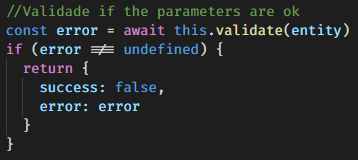
\includegraphics[scale=1.60]{./Figuras/code/server/controller-class-validator.png}
	\end{center}
	\legend{Fonte: Próprio Autor, 2019}
\end{figure}

A figura \ref{code_server_class-validate} mostra a aplicação da validação da biblioteca \textit{class validator}.

\newpage
\subsection{Middleware: Validação do JWT}

\begin{figure}[htb]
	\caption{\label{code_server_middleware}Middleware: Validação do JWT}
	\begin{center}
		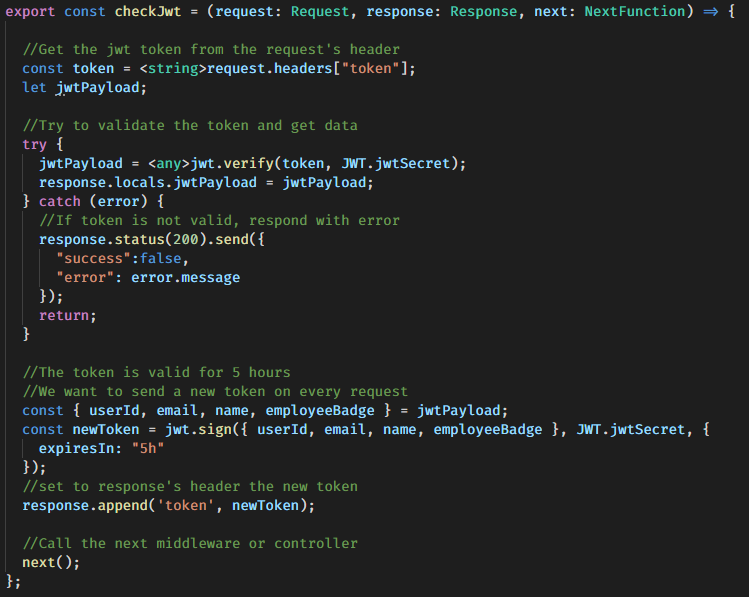
\includegraphics[scale=0.80]{./Figuras/code/server/middleware.png}
	\end{center}
	\legend{Fonte: Próprio Autor, 2019}
\end{figure}

A figura \ref{code_server_middleware} mostra a validação do token e a estratégia de renovação do token enviado.

\newpage
\subsection{TypeOrm: Query as Function}

\begin{figure}[htb]
	\caption{\label{code_server_typeorm-query-as-function}TypeOrm: Query as Function}
	\begin{center}
		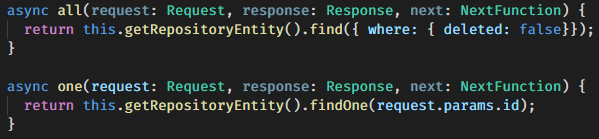
\includegraphics[scale=1.00]{./Figuras/code/server/typeorm-query-as-function.png}
	\end{center}
	\legend{Fonte: Próprio Autor, 2019}
\end{figure}

A figura \ref{code_server_typeorm-query-as-function} mostra interação com o banco de dados montada pela ORM e disponibilizada como função.

\subsection{Estratégia de Exclusão de Dados}

\begin{figure}[htb]
	\caption{\label{code_server_delete-strategy}Estratégia de Exclusão de Dados}
	\begin{center}
		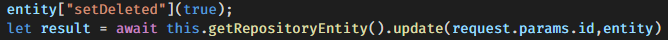
\includegraphics[scale=0.90]{./Figuras/code/server/delete-strategy.png}
	\end{center}
	\legend{Fonte: Próprio Autor, 2019}
\end{figure}

A figura \ref{code_server_delete-strategy} mostra a estratégia adotada para exclusão de resgistros, onde o registro não será realmente deletado, apenas irá alterar o atributo ''deleted'' para true. Desta maneira poderemos rapidamente desfazer uma exclusão errada e não teremos problemas com histórico apagado das entidades.
